\documentclass{article}
\usepackage[a4paper,left=1in, right=1in, top=1in, bottom=1in]{geometry}
\usepackage{hyperref}
\usepackage{graphicx}
\usepackage{wrapfig}
\usepackage{footnote}
\DeclareGraphicsExtensions{.pdf,.png,.jpg}
\graphicspath{ {./images/} }
\begin{document}
\title{Single Battery Charge Test}
\date{}
\maketitle
\section{Goal}
Safely charge 1 Li-Ion battery through multiple charge test cycles using the Gibbot v4 charge test board, which uses the LTC4000 charge controller and the LT1704 DC/DC Converter. 

\subsection{Procedure}
According to the specification sheet for the Tenergy LiFePO4 3.2V 1100mAh 18650 Battery\footnote{http://www.all-battery.com/datasheet/30072-0\_datasheet.pdf} the charge voltage of the battery is 3.6V$\pm$0.05V, the average working voltage is 3.2V, the standard charge current is 0.5A and the standard discharge end voltage is 2.0V. The measured storage voltage for the batteries is 3.30V. 
For initial tests the battery will be discharged through a power resistor from 3.30V to 3.0V. The charger will then charge the battery back up to 3.60V.

The following outputs will be measured with an oscilloscope during charging:
\begin{description}
\item[$\mathbf{V_{OUT}}$] Gives the voltage of the battery
\item[IIMON] The voltage on this pin is 20 times (typical) the sense voltage $V_{IN,CLN}$across the input current sense resistor $R_{IS}$, therefore providing a voltage proportional to the input current.
\item[IBMON] The voltage on this pin is 20 times (typical) the sense voltage $V_{IN,CLN}$across the charge current sense resistor $R_{IS}$, therefore providing a voltage proportional to the charge current.
\end{description}

\section{Program Resistor Values}
\begin{figure}[h]
\centering
\caption{LTC 4000 Footprint}
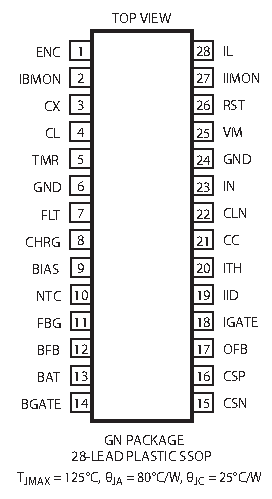
\includegraphics[width=.25\textwidth]{footprint}
\end{figure}
The \href{http://cds.linear.com/docs/en/datasheet/4000fa.pdf}{LTC4000} is a charge controller that interfaces with a DC/DC Buck Converter to regulate the voltage input to the main board  and the charging circuit. The \href{http://cds.linear.com/docs/en/datasheet/4000fa.pdf}{LTC4000} has 4 regulation loops for
\begin{enumerate}
\item Input current control
\item Battery current control when the battery is charging and trickle charging
\item Battery voltage control
\item Output voltage control
\end{enumerate}
Threshold values for each of these regulation loops are set using resistor divider networks. 

\subsection{Programmed Voltage Levels}
Translating the specs above into the values used by the LTC4000 we get:
\[V_{FLOAT} = 3.6V\]
\[V_{OUT} = 4.0V\]
These values satisfy the qualification from the datasheet that "$V_{OUT}$ should not be programmed to be less than 105\% of $V_{FLOAT}$ to ensure that the battery can be fully charged\footnote{pg 20 http://cds.linear.com/docs/en/datasheet/4000fb.pdf}." They are also in line with the Design Example modified for a single LiFePO4\footnote{pg 20 http://cds.linear.com/docs/en/datasheet/4000fb.pdf}.\\ \\
Setting $V_{OUT}$ automatically sets $V_{OUT(INST\_ON)}$ as\footnote{pg 20 http://cds.linear.com/docs/en/datasheet/4000fb.pdf}:
 
\[V_{OUT(INST\_ON)} = \frac{V_{OUT}}{1.225} = 3.27V\]\\
Setting $V_{FLOAT}$ automatically sets $V_{LOBAT}$  as\footnote{LTC4000 Datasheet, Electrical Characteristics, pg3 http://cds.linear.com/docs/en/datasheet/4000fb.pdf}:
\[V_{LOBAT} = V_{FLOAT}*0.68 = 2.45V\]

$V_{OUT(INST\_ON)}$ sets a battery voltage level for which the charger will regulate the MOSFET at BGATE. If a battery is connected with a voltage below $V_{OUT(INST\_ON)}$ BGATE is regulated to ensure that the voltage at the output is maintained at the level of $V_{OUT(INST\_ON)}$. For this reason $V_{OUT(INST\_ON)}$ should be programmed to be the minimum output voltage required to power the output.

It is important to not set $V_{OUT}$ too high relative to $V_{FLOAT}$. From the datasheet "$V_{OUT}$ should not be programmed too high since $V_{OUT(INST\_ON)}$, the minimum 
voltage on CSP, depends on the same resistors $R_{OFB1}$ and 
$R_{OFB2}$ that set $V_{OUT}$...The higher the programmed value of 
$V_{OUT(INST\_ON)}$, the larger the operating region when the 
charger PMOS is driven in the linear region where it is 
less efficient\footnote{pg 20 http://cds.linear.com/docs/en/datasheet/4000fb.pdf}." 


\subsection{$\mathbf{R_{OFB1} = 298k\Omega}$ \& $\mathbf{R_{BFB1}=288k\Omega}$}
$V_{OUT}$ is set by a resistor divider from CSP to FBG with the junction connected to OFB. $R_{OFB2}$, the resistor between FBG and OFB, will have the datasheet recommended value of 127k\footnote{Typical Application circuit diagram pg 1 LTC4000 datasheet http://cds.linear.com/docs/en/datasheet/4000fb.pdf}. The value of $R_{OFB1}$ is set using the formula\footnote{pg 18 LTC4000 datasheet http://cds.linear.com/docs/en/datasheet/4000fb.pdf}:

\[R_{OFB1} = \left ( \frac{V_{OUT}}{1.193} - 1 \right)  \cdot 127k\Omega=\left ( \frac{4.0V}{1.193} - 1 \right)\cdot 127k\Omega = 298k\Omega\]
$V_{FLOAT}$ is set by a resistor divider from BAT to FBG with the junction connected to BFB. $R_{BFB2}$, the resistor between FBG and BFB, will have the datasheet recommended value of 133k\footnote{Typical Application circuit diagram pg 1 LTC4000 datasheet http://cds.linear.com/docs/en/datasheet/4000fb.pdf}. For the float voltage of 3.6V from above, the value of $R_{BFB}$ is set using the formula\footnote{pg 17 LTC4000 datasheet http://cds.linear.com/docs/en/datasheet/4000fb.pdf}: 
\[R_{BFB1} = \left ( \frac{V_{FLOAT}}{1.135} - 1 \right ) \cdot 133k\Omega = \left ( \frac{3.6V}{1.135} - 1 \right ) \cdot 133k\Omega  = 288k\Omega\]

\subsection{$\mathbf{R_{IL}=1k\Omega}$ \& $\mathbf{R_{CL}=1k\Omega}$}
Both $R_{IL}$ and $R_{CL}$ should be set to 2k to limit both the input current and the charge current to a maximum value of 0.5A according to the following formula\footnote{From pg 16  of the LTC4000 datasheet http://cds.linear.com/docs/en/datasheet/4000fb.pdf}:

\[R_{IL} = \frac{I_{LIM} \cdot R_{IS}}{2.5uA} = \frac{0.5A\cdot5m\Omega}{2.5uA}=1k\Omega\]
\[R_{CL} = \frac{I_{CLIM} \cdot R_{CS}}{2.5uA} =\frac{0.5A\cdot5m\Omega}{2.5uA}=1k\Omega\]
Assuming the sense resistor for both is a \href{http://www.digikey.com/product-detail/en/PWR4412-2SCR0050F/PWR4412-2SCR0050F-ND/2564433}{5m$\Omega$, 1\% accuracy, 3W, metal element sense resistor}. If a power resistor is applied between $V_{OUT}$ and GND the current through the resistor should be subtracted from the charge current. This difference can be measured in the difference of the voltage outputs between IIMON and IBMON.

\subsection{$\mathbf{C_{TMR}=8nF}$ \& $\mathbf{R_{CX}=2k\Omega}$}
After the float voltage is reached the charger starts a timer. When this timer runs out the charge stops chargin. The period of time for which the batteries will trickle charge is set by $C_{TMR}$ according to the following formula\footnote{From pg 18 of the LTC4000 datasheet http://cds.linear.com/docs/en/datasheet/4000fb.pdf}.
\[C_{TMR} = t_{TERMINATE}(h) \cdot 34.6nF = 0.25h \cdot 34.6nF = 8.65nF\]
This also sets the period of time for which the charger will supply current to a battery whose voltage is below the Bad Battery Voltage. 

\[t_{BADBAT} = \frac{C_{TMR}(nF)}{138.5} = \frac{8nF}{138.5}= 3.5min\]
If TMR were instead tied to BIAS charge termination is controlled by $R_{CX}$ according to the following formula. Where $I_{CX}$ is used for C/10 charging.

\[R_{IL} = \frac{I_{C/X} \cdot R_{CS}+0.5mV}{0.25uA} = \frac{.05A\cdot5mOhm + 0.5mV}{.25uA}=2k\Omega\]
Because a capacitor is connected between TMR and GND the capacitor ($C_{TMR}$) controls charge termination. In this configuration, the only effect $R_{CX}$ will have is that the outputs of CHRG and FLT will assume a high impedance state when the charge current falls below$I_{C/X}$ \footnote{From pg 18  of the LTC4000 datasheet http://cds.linear.com/docs/en/datasheet/4000fb.pdf}. Because CHRG and FLT are not properly connected on this board, this effect cannot be observed. 

\subsection{FLT \& CHRG Shorterd}
FLT and CHRG were supposed to be connected to LEDs to indicate an over temperature condition or an active charge cycle. However, the LEDs are connected to ground and the outputs are only pull down outputs. Either rewire the anode of the diodes to a high voltage source and change the resistor values or short the outputs to GND.

\subsection{$\mathbf{R_{VM1}}$}
The input voltage pin VM measures the input voltage through a voltage divider. If the input voltage level drops below a given threshold the controller will pull the RST pin low. If this pin were connected to the EN of a buck converter it would disable the buck converter and cut power to the batteries and VOUT. An LED could also be connected to the RST pin so that instead of shutting down the buck converter, the LED would provide a visual indicator if the voltage is too low. Because the RST pin is left unconnected in this iteration the input voltage level set on pin VM will have no effect, but will be configured anyway. 

The minimum supplied voltage required to charge the circuit can be calculated from the LT1074 datasheet based on the equation below\footnote{LT1074 Design Manual Application Note 44, Pg 17, Equation 1 http://cds.linear.com/docs/en/application-note/an44fa.pdf} and the limitation that the maximum duty cycle is 90\%\footnote{Listed as 90\% in electrical characteristics table pg 4. Stated as 93\% on pg 6. http://cds.linear.com/docs/en/application-note/an44fa.pdf}. 
\[V_{IN} = \frac{V_O + V_f}{90\%} + V_{SW} =  \frac{4.0V + 0.48V}{90\%} + 2V = 7.0V\]
Where:

$V_{SW}$ = Switching voltage of LT1074 ~ 2V

$V_{f}$ = Diode forward voltage = 0.48V for PDS760\\

The voltage is set by a voltage divider from the input voltage source to GND with VM connected at the junction. The value of R2, the resistor from VM to GND is set to 100k according to the datasheet\footnote{Typical Application circuit diagram pg 1 LTC4000 datasheet http://cds.linear.com/docs/en/datasheet/4000fb.pdf}. The value of $R_{VM1}$ is set using the equation below\footnote{LTC4000 datasheet pg 23 http://cds.linear.com/docs/en/datasheet/4000fb.pdf}.

\[R_{VM1} = \left (\frac{V_{VM\_RST}}{1.193V}-1\right )\cdot R_{VM2} = \left (\frac{7.0V}{1.193V}-1\right )\cdot 100k = 487k\Omega\]

\subsection{NTC}
Temperature qualification is unnecessary in this test. Leave NTC, 21.6k and 9.91k unsoldered. 

\subsection{LT1074 FB1}
The datasheet recommends that the DC/DC Converter should be set to regulate it's output voltage at greater than 110\% of the output voltage\footnote{LTC4000 Datasheet pg 23 http://cds.linear.com/docs/en/datasheet/4000fb.pdf}. For the output voltage of $V_{OUT} = 4.0V$ above this means the LT1074 should be programmed to output at least 4.4V. 

The value of $R_{FB2}$ is set to the datasheet recommended value of 2.21k$\Omega$. The value of $R_{FB1}$ is set according to the following formula:
\[ R_1 = \frac{R_2 \cdot (V_{OUT} - V_{REF})}{V_{REF}} = \frac{2.21k\Omega \cdot (4.0V - 2.21V)}{2.21V} = 1.79k\Omega\]

\subsection{LT1074 FDBK $\mathbf{R_C}$ \& $\mathbf{C_C}$}
For the final circuit the loop compensation resistor and capacitor values should be determined either emperically or analytically. For this initial test they will be set at the datasheet recommended initial value of $C_C$ = 1uF and $R_C$ = 10k will be used.
\section{PCB Components}

\subsection{MOSFETs}
Two P-Channel MOSFETs control the flow of current. A MOSFET between IID and CSP controls the flow of power from the input source. A MOSFET between CSN and BAT controls the power flowing in and out of the batteries. 

\subsubsection{Input Power Control}
The parameters that determine the choice of MOSFET are: 
\begin{itemize}
\item The maximum drain to source voltage is 10*3.6*1.05 = 37.8V
\item The drain to source current is 5A
\item An acceptable temperature rise is 30 C during operation
\end{itemize}
These parameters led to the choice of \href{http://www.vishay.com/docs/72439/72439.pdf}{Vishay's SUM110P06-07L} which can tolerate 60V D-S. If $V_{GS} = 4.5V$, $R_{DS(on)} = 8.8mOhm$ at ambient temperature. When the MOSFET is passing 5A it will be dissipating 0.22W. With an $R_{\Theta JA}$of 40 C/W the junction temperature would only rise by about 9 C.

\subsubsection{Battery Power Control}
The BGATE MOSFET is limited by the power it must dissipate during charging. When the battery voltage is below $V_{INST\_ON}$ = 3.27V, the BGATE MOSFET is regulated to maintain a steady output voltage. However, this means that the MOSFET is being used as a resistor and will dissipate more power. The power dissipated when the battery is below $V_{LOBAT}$ and the charger is trickle charging is calculated using the following equation\footnote{LTC4000 Datasheet pg 19, 27 http://cds.linear.com/docs/en/datasheet/4000fb.pdf}:
\[P_{TRKL} = (0.86*V_{FLOAT} - V_{BAT})*I_{CLIM(TRKL)} = (0.86*3.6V - 0V)*0.05A = 0.15W\]
Where:

$I_{CLIM(TRKL)} = I_{CLIM}/10 = 0.05A$\\

The power dissipation when the battery voltage is above $V_{LOBAT}$, but below $V_{INST\_ON}$ is calculated using\footnote{LTC4000 Datasheet pg 19, 27 http://cds.linear.com/docs/en/datasheet/4000fb.pdf}:

\[P_{INST\_ON} = (0.86*V_{FLOAT} - V_{BAT})*I_{CLIM}= (0.86*3.6V - 2.45V)*0.5A = 0.49W\]

Power dissipation will not be an issue in this setup, but should be considered when more batteries or higher charge current are implemented. The other parameters determining the choice of BGATE MOSFET are looser than the parameters for the IGATE MOSFET:
\begin{itemize}
\item The maximum drain to source voltage is 10*3.6 = 36V
\item The drain to source current is 4A
\end{itemize}
However, to simplify the design, \href{http://www.vishay.com/docs/72439/72439.pdf}{Vishay's SUM110P06-07L} MOSFET will be used in both locations. This could be reconsidered in future designs to save space--move from a D2PAK to a DPAK MOSFET--or to reduce the $R_{DS(ON)}$ on the $B_{GATE}$ MOSFET.

\end{document}